\documentclass[20pt]{article}
\usepackage[utf8]{inputenc}
\usepackage{amsmath}
\usepackage{amssymb}
\usepackage{amsfonts}		 
\usepackage{enumitem}
\usepackage{fancyheadings}
\usepackage{mathtools}
\usepackage{tikz}
\usetikzlibrary{automata,positioning}
\DeclarePairedDelimiter{\ceil}{\lceil}{\rceil}
\DeclarePairedDelimiter\floor{\lfloor}{\rfloor}
\usepackage[margin=3cm]{geometry}

\title{CSC236H1 Assignment 2}
\author{Martin Chak and Tony Yang}
\date{November 11, 2019}

\begin{document}

%BEGIN TITLE PAGE

\maketitle

%END TITLE PAGE

\newpage

%BEGIN Q1
\section*{Question 1}

\begin{text}
    For each of the following, decide if the statement is true and justify your answer
\end{text}

\begin{enumerate}[label=(\alph*),leftmargin=0cm]
    \item \text{If $L(R)$ \subseteq \, $L(S)$, then \, $R^* + S^* \equiv (R + S)^*$}
    \item \text{If $L(R)$ \subseteq \, $L(S)$, then \, $R^*S^* \equiv (RS)^*$}
\end{enumerate}

\noindent
\begin{enumerate}[label=(\alph*),leftmargin=0cm]
    \item 
    \begin{text}
        We want to prove that for arbitrary regular expressions $R$ and $S$ that if $L(R)$ \subseteq \, $L(S)$, then \, $R^* + S^* \equiv (R + S)^*$.\\
        We let $R$ and $S$ be arbitrary regular expressions such that $L(R) \subseteq \, L(S)$ hold. Then:
    \end{text}
    \begin{align}
        L(R^*+S^*) &= \bigcup\limits_{{k} \in \mathbb{N}} L(R)^{k} + \bigcup\limits_{{k}\in \mathbb{N}} L(S)^{k}\\
        L((R+S)^{*}) &= \bigcup\limits_{{k} \in \mathbb{N}} {L(R + S)^{k}}
    \end{align}
    \begin{text}
        We will use induction to show $P(k):$ Statement $(1)$ is equal to $(2)$ for $k$ unions in the statement\\
        \textbf{Base case (k = 0):} $P(k)$ holds since both $(1)$ and $(2)$ are empty.\\
        \textbf{Induction step:} Assume $P(k)$ holds for $k\in\mathbb{N}$, we want to prove $P(k+1)$ holds. Thus:
    \end{text}
    \begin{align}
        \bigcup\limits_{{k} \in \mathbb{N}} L(R)^{k+1} + \bigcup\limits_{{k}\in \mathbb{N}} L(S)^{k+1} &= \{L(R) + L(S)\} \circ \{L(R)^2 + L(S)^2\}\circ...\nonumber\\
        \bigcup\limits_{{k} \in \mathbb{N}} {L(R + S)^{k+1}} = \{L(R + S)\} \circ \{L(R + S)^2\}\circ... &= \{L(R) + L(S)\} \circ \{L(R)^2 + L(S)^2\}\circ...\nonumber
    \end{align}
    \begin{text}
        Thus we have shown $P(k+1)$ holds and therefore the two statements are equivalent
        
        \hfill $\blacksquare$
    \end{text}
    
    \item
    \begin{text}
        We want to disprove this statement, we first define a language $L(S)$, where $S = (1)(0+1)^*$ so that $L(S)$ represents a language of binary strings that starts with $1$, and we define a second language $L(R)$, where $R = (11)(0+1)^*$ so that $L(R)$ represents a language of binary string that starts with $11$. Thus we know $L(R) \subseteq \, L(S)$ since all elements in $L(R)$ start with a $1$, but not all strings in $L(S)$ start with $11$, thus every element in $L(R)$ is in $L(S)$ but the converse is not true.\\
        
        Therefore we can disprove $R^*S^* \equiv (RS)^*$ by showing an element that appears in one statement and not in the other, and this is evident since we can let:
    \end{text}
    
    \begin{equation}
        w = (\varepsilon)(1) \in R^{*}S^{*} \tag{Since, $\varepsilon \in R^*$ and $1 \in S^{*}$}
    \end{equation}
    
    \begin{text}
        However, the above string cannot be an element of $(RS)^{*}$, since $1 \notin (RS)^{*}$ as the smallest string in $R$ is $11$, therefore no matter what string in $S$ we pick, the string in $w \in R^{*}S^{*}$ is not in $(RS)^{*}$.\\
        
        To conclude, we have shown that the two sets are not equivalent by showing an element that is in one of the sets, but not the other.\\
        
        \hfill $\blacksquare$
    \end{text}
\end{enumerate}

%END Q1

\newpage

%BEGIN Q2
\section*{Question 2}

\begin{text}
    Construct a DFA $D$ with 5 states such that $D$ only accepts dyadic strings whose values are multiples of 5, such that:
\end{text}

\begin{equation}
    L(D) = \{w \in \{1,2\}^{*}:(val(w) \% 5) = 0\} \nonumber
\end{equation}

\begin{center}
    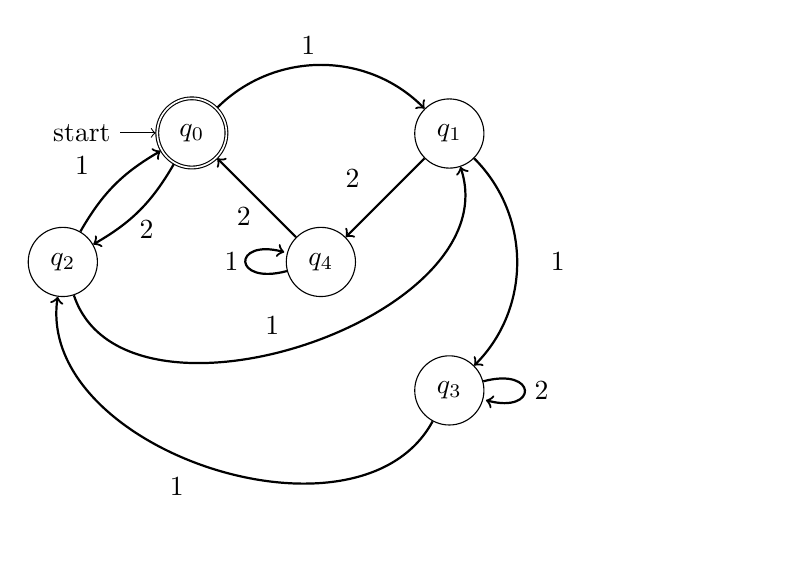
\begin{tikzpicture}
        \node[state, initial, accepting] (q_0) {$q_0$};
        \node[state] (q_2) [below left = of q_0] {$q_2$};
        \node[state] (q_4) [below right = of q_0] {$q_4$};
        \node[state] (q_1) [above right = of q_4] {$q_1$};
        \node[state] (q_3) [below right = of q_4] {$q_3$};
        
        %0 to 1 with 1
        \draw[thick, ->] (q_0) edge[bend left = 45] node [text width=2.5cm,right= 1cm, midway,above] {$1$} (q_1);
        
        %0 to 2 with 2
        \draw[thick, ->] (q_0) edge[bend left = 15] node [text width=2.5cm,right= 1.25cm, midway,below] {$2$} (q_2);
        
        %1 to 3 with 1
        \draw[thick, ->] (q_1) edge[bend left = 45] node [text width=2.5cm,right= 0.3cm, midway] {$1$} (q_3);
        
        %1 to 4 with 2
        \draw[thick, ->] (q_1) -- node [text width=2.5cm,right= 0.75cm, midway,above] {$2$} (q_4);
        
        %2 to 0 with 1
        \draw[thick, ->] (q_2) edge[bend left = 15] node [text width=2.5cm,right= 0.75cm, midway,above] {$1$} (q_0);
        
        %2 to 1 with 2
        \draw[thick, ->] (q_2) edge[bend right = 90] node [text width=2.5cm,right= 0.75cm, midway,above] {$1$} (q_1);
        
        %3 to 2 with 1
        \draw[thick, ->] (q_3) edge[bend left = 80] node [text width=2.5cm,right= 0.75cm, midway,below] {$1$} (q_2);
        
        %3 to 3 with 2
        \draw[thick] (q_3) edge[loop right] node [text width=2.5cm, midway, right] {$2$} (q_3);
        
        %4 to 4 with 1
        \draw[thick] (q_4) edge[loop left] node [text width=2.5cm, midway, right= -0.4cm] {$1$} (q_4);
        
        %4 to 0 with 2
        \draw[thick, ->] (q_4) -- node [text width=2.5cm,right= 1cm, midway,below] {$2$} (q_0);
    \end{tikzpicture}
    
    %State Invariants
    \begin{equation}
    \delta^{*}(q_0, w)
    \begin{cases}
      q_0, & \text{iff w is empty or w's value is a multiple of 5}\nonumber\\
      q_1, & \text{iff the remainder of the value of w divided by 5 is 1}\nonumber\\
      q_2, & \text{iff the remainder of the value of w divided by 5 is 2}\nonumber\\
      q_3, & \text{iff the remainder of the value of w divided by 5 is 3}\nonumber\\
      q_4, & \text{iff the remainder of the value of w divided by 5 is 4}\nonumber\\
    \end{cases}
  \end{equation}
\end{center}

%END Q2

\newpage

%BEGIN Q3
\section*{Question 3}

\noindent
\section*{\normalfont{3a i) $L(0^*1^*00^*)$ with three states}}
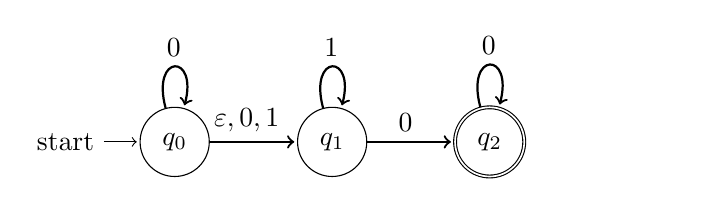
\begin{tikzpicture} [shorten >=1pt,node distance=2cm,on grid,auto] 
    \node[state, initial] (a) {$q_0$};
    \node[state] (b) [right= of a] {$q_1$};
    \node[state, accepting] (c) [right= of b] {$q_2$};
    
    \draw[thick] (a) edge[loop above] node [text width=2.5cm,right= 1.15cm, midway,above] {$0$} (a);
    \draw[thick, ->] (a.east) -- node [text width=2.5cm,right= 0.75cm, midway,above] {$\varepsilon, 0, 1$} (b.west);
    \draw[thick] (b) edge[loop above] node [text width=2.5cm,right= 1.15cm, midway,above] {$1$} (b);
    \draw[thick, ->] (b.east) -- node [text width=2.5cm,right= 1.1cm, midway,above] {$0$} (c.west);
    \draw[thick] (c) edge[loop above] node [text width=2.5cm,right= 1.15cm, midway,above] {$0$} (c);
\end{tikzpicture}



\noindent
\section*{\normalfont{\indent\, ii) $L(1^*(0011^*+011^*)^*)$ with three states}}

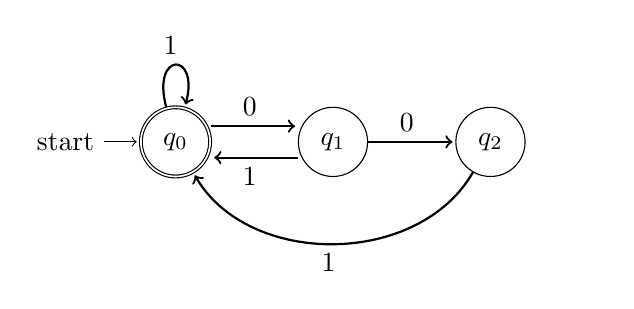
\begin{tikzpicture} [shorten >=1pt,node distance=2cm,on grid,auto] 
    \node[state, initial, accepting] (a) {$q_0$};
    \node[state] (b) [right= of a] {$q_1$};
    \node[state] (c) [right= of b] {$q_2$};
    
    \draw[thick] (a) edge[loop above] node [text width=2.5cm,right= 1.1cm, midway,above] {$1$} (a);
    \draw[thick, ->] ([yshift = 0.2cm]a.east) -- node [text width=2.5cm,right= 1.1cm, midway,above] {$0$} ([yshift = 0.2cm]b.west);
    \draw[thick, ->] ([yshift = -0.2cm]b.west) -- node [text width=2.5cm,right= 1.1cm, midway,below] {$1$} ([yshift = -0.2cm]a.east);
    \draw[thick, ->] (b.east) -- node [text width=2.5cm,right= 1.1cm, midway,above] {$0$} (c.west);
    \draw[thick, ->] (c) edge[bend left = 60] node [text width=2.5cm,right= 1.1cm, midway,below] {$1$} (a);
\end{tikzpicture}


\noindent
\section*{\normalfont{\normalfont{3b i) $\{w \in \{0,1\}^{*} : $ every odd position of $w$ is a $1\}$}}}

\begin{equation}
    ((1)(0+1))^*(1 + \varepsilon)\nonumber
\end{equation}
\begin{enumerate}[label=\alph*]
    \item 
    The $((1)(0+1))^*$ part ensures that our string has 1 on odd positions and either 0 or 1 on even positions. 
    \item
    The $(1 + \varepsilon)$ part ensures that we can either have a single 1 or an empty string if the first part is empty (the empty string is considered part of the language because there does not exist a 1 that is not in the odd position for the empty string). If the first part is non-empty, we can ensure that the string ends with either a 1 or an empty string, which is in an odd position.
\end{enumerate}


\noindent
\section*{\normalfont{\indent\, ii) $\{w \in \{0,1\}^{*} : w $ does not end in $100\}$}}

\begin{equation}
    ((0 + 1 + \varepsilon)(0 + 1 + \varepsilon) + (0 + 1)^*(000 + 001 + 010+ 011 + 101 + 110+ 111))\nonumber
\end{equation}

\begin{enumerate} [label=\alph*]
    \item 
    The $(0 + 1 + \varepsilon)(0 + 1 + \varepsilon)$ part represents all the strings less than length of 3 that belongs to the language. $(\varepsilon, 0, 1, 00, 01, 10, 11)$
    \item
    The $(0 + 1)^*(000 + 001 + 010+ 011 + 101 + 110+ 111)$ part represents all the strings with length greater than or equal to 3 that belongs to the language. We specified the suffix so 100 is not included.
\end{enumerate}



%END Q3

\newpage

%BEGIN Q4
\section*{Question 4}
\begin{text}
    Let $L$ be and arbitrary regular language defined over an alphabet $\Sigma$. Construct an FSA for $Rev(L)$ (reversal of language $L$) and prove its correctness. We define:
    
    \noindent
    Let $D_L = <Q_L, \Sigma_L, \delta_L, q_L, F_L>$ such that $D_L$ is a DFA and $L = L(D_L)$\\
    Let $N_R = <Q_R, \Sigma_R, \delta_R, s, F_R>$ such that $N_R$ is an NFA where $Rev(L) = L(N_R)$\\
    We define the initial state of $N_R$ as $s$ such that $\delta_F(s,\varepsilon) \in F_L$ since we can have more than one accepting state in the language $L$. We also define the alphabet $\Sigma_R = (\Sigma_L)^R$, $Q_R = Q_L \cup \{s\}$ and $F_R = \{q_L\}$. We then define the transition states as:
\end{text}

\begin{equation}
    \delta_R^{*}(q, c) =
    \begin{cases}
      p_i \in F_L, & \text{iff $q = s$ and $c = \varepsilon$}\nonumber\\
      p \text{ where q = $\delta_L^*(p, c)$}, & \text{otherwise}\nonumber\\
    \end{cases}
\end{equation}

\noindent
\begin{text}
    In order to prove the above we want to prove the following predicate, that $\forall w \in \Sigma_R^*$ and $\forall p_L, p_R \in Q_L$
\end{text}

\begin{equation}
    P(w): p_R = \delta_L^*(p_L, w) \iff p_L = \delta_R^*(p_R, w^R)\nonumber
\end{equation}

\noindent
\begin{text}
    \noindent
    \textbf{Base Case ($w=\varepsilon$):}\\
    Let $w = \varepsilon$ and $p_L, p_R \in Q_L$, we want to show $P(\varepsilon)$, such that $p_R = \delta_L^*(p_L, \varepsilon) \iff p_L = \delta_R^*(p_R, \varepsilon^R)$ holds. Since $w = \varepsilon$, we know $w = w^R$, since $\varepsilon = \varepsilon^R$. Then let $p_L$ and $p_R$ be states such that $p_R = \delta_L^*(p_L, \varepsilon)$. But by definition, $\delta_L^*(p_L, \varepsilon) = p_L$, thus $p_L = p_R$ and then the converse is true if we assume the right side. As an edge case, if $p_L, p_R \in F_L$, then for the right side: $\delta_R(p_R, \varepsilon) \in F_L$, by definition of $\delta_R^*(q,c)$, so that $p_L$ can equal $p_R$ since $F_L \subseteq Q_L$. Thus the base case is true.
\end{text}

\noindent
\begin{text}
    \noindent
    \textbf{Induction Step:}\\
    Let $w \in \Sigma_R^*$, such that $w = ua$, where $u \in \Sigma_R^*$ and $a \in \Sigma_R$. We assume $P(u)$ holds (I.H.) and we will use this to prove $P(w): p_R = \delta_L^*(p_L, w) \iff p_L = \delta_R^*(p_R, w^R)$, holds. We start by assuming the left side:
\end{text}

\begin{align}
    p_R = \delta_L^*(p_L, w) &\iff p_R = \delta_L^*(p_L, ua)\nonumber\tag{By definition of $w$}\\
    &\iff p_R = \delta_L(\delta_L^*(p_L, u), a)\nonumber\\
    &\iff p_R = \delta_L(p_w, a)\nonumber\tag{By I.H. $\exists p_w$ s.t. $p_w = \delta_L^*(p_L,u)$}\\
    &\iff p_w = \delta_R(p_R, a)\nonumber\tag{By construction of $\delta_R^*$}\\
    &\iff \delta_L^*(p_L, u) = \delta_R(p_R, a)\nonumber\tag{By I.H. again}\\
    &\iff p_L = \delta_R^*(\delta_R(p_R, a), u^R)\nonumber\\
    &\iff p_L = \delta_R^*(p_R, au^R)\nonumber\\
    &\iff p_L = \delta_R^*(p_R, w^R)\nonumber\tag{$w=au^R$}
\end{align}

\noindent
\begin{text}
    Therefore $\forall w \in \Sigma_R^*$, $P(w)$ holds. And the same for $w \in \Sigma_L^*$ since $\Sigma_L^* = \Sigma_R^*$.\\
\end{text}

\noindent
\begin{text}
    Now suppose $w \in \Sigma_R^*$. Then:
\end{text}
\begin{align}
    w \in L &\iff w = x^R\text{ and }x \in \L\nonumber\\
    &\iff w = x^R\text{ and }\delta_L^*(q_L, x) \in F_L\nonumber\\
    &\iff w = x^R\text{ and }\delta_R^*(q_R, x^R) \in F_R\nonumber\tag{Since $P(w) holds$}\\
    &\iff w = x^R\text{ and }\delta_R^*(\delta(s,\varepsilon), x^R) \in F_R\nonumber\tag{Since we know $\delta(s,\varepsilon) \in F_L$}\\
    &\iff w = x^R\text{ and }\delta_R^*(s, x^R) \in F_L\nonumber\\
    &\iff \delta_R^*(s, w) \in F_L\nonumber
\end{align}

\noindent
\begin{text}
    Therefore, $N_R$ only accepts reversed strings of the regular language $L$, thus $L^R$ is a regular language.
\end{text}

\hfill $\blacksquare$
%END Q4

\newpage

%BEGIN Q5
\section*{Question 5}
\begin{text}
    Consider $L = \{0^{n}1^{m}2^{n-m}:n \geq m \geq 0,$ where $n,m\in\mathbb{N}\}$. Use the Pumping Lemma to prove that $L$ is not regular.\\\\

    \noindent
    Assume for contradiction that $L$ is regular so that $\exists p \geq 1$ s.t. $\forall w \in L$ with $|w| \geq p$ so there are strings $x,y,z$ s.t. the following hold
\end{text}

\noindent
\begin{enumerate}
    \item $w=xyz$
    \item $|y| \geq 1$
    \item $|xy| \leq p$
    \item $\forall i \geq 0, xy^{i}z \in L$
\end{enumerate}

\noindent
\begin{text}
    Assume 1 through 3 hold. Let $w = 0^{p}1^{k}2^{p-k}$ so that $w \in L$ and $|w| = 2p$. We pick $x$,$y$ and $z$ such that $w=xyz$, so $x = 0^0$, $y=0^p$, $z = 1^k\cdot2^{p-k}$. Since $p \geq 1$ then $|y| \geq 1$ as $|y| = p$ so  1 and 2 hold, and since $|xy| = |y|$, then $|xy| \leq p$ since $|xy| = p$, thus 3 holds.\\
    
    \noindent
    But then for any $i \geq 0$, $xy^{i}z \in L$ should hold. But if we let $i = 2$, by assumption, then $xy^2z \in L$ must hold. However, that means that $0^{2p} \cdot 1^{k} \cdot 2^{p-k} \in L$ must hold. But this new string cannot be in L, since by definition of the language $L$, in order for there to be $2p$ $0$'s and $k$ $1$'s, there must be $2p-k$ $2$'s for the string to be an element of $L$. But our new string only has $p-k$ $2$'s and thus contradicts our assumption that $L$ was a regular language, consequently proving that $L$ is a non-regular language.
\end{text}

\hfill $\blacksquare$

%END Q5

\end{document}
